\chapter{Auswertung}
\label{chap:auswertung}
% =================================================================
\thispagestyle{fancy}
% =================================================================
\section{Beugung am Spalt und Antispalt}
Hier wurden die Maximas, resp. die Minimas beim Interferenzmuster auf dem Schirm gemessen. Mithilfe der Gleichung \ref{eq:1} wurde dann die Spalt-, resp. die Antispaltbreite mit QTI-Plot gefittet und graphisch dargestellt. Die Wellenlänge l des He-Ne-Lasers wurde jeweils direkt in der Formel mit 6.328e-07 m, sowie die Brennweite f resp. der Abstand des Spaltes zum Schirm L eingetragen.\\
\vspace{-0.5cm}
%******************************************
\begin{figure}[h]
\centering
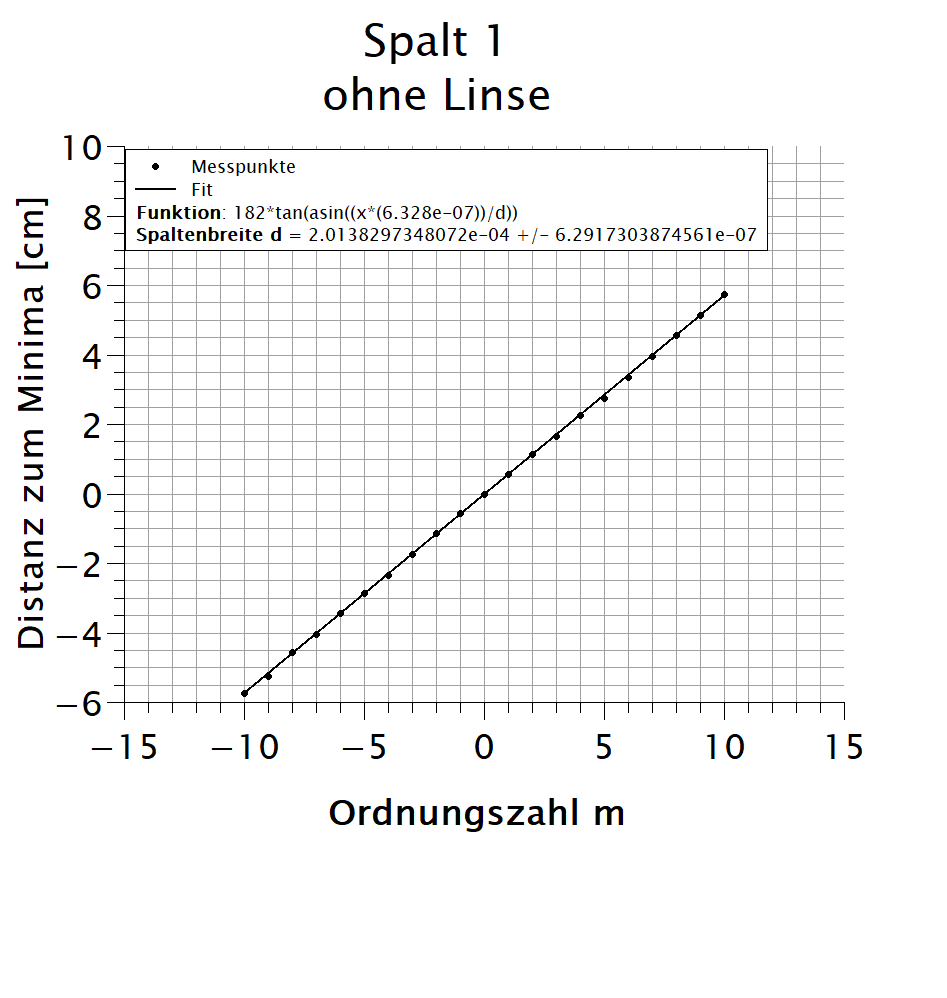
\includegraphics[width=\textwidth]{Bilder/spalt1_ohneLinse.png}
\vspace*{-3.5cm}
\caption[Spalt 1: ohne Linse]{Hier wird der Abstand vom Mittelpunkt zum Minima des Interferenzmusters bei bestimmter Ordnungszahl, direkter Beobachtung und ohne Linse dargestellt. Dabei wird, wie in der Legende zu sehen ist, die Spaltenbreite mit ihrem Fehler gefittet. Es wurde zum Fit die Distanz vom Objekt zum Schirm von 182cm verwendet.}
\label{fig:spalt1_ohneLinse}
\end{figure}
\newpage
%============================================
\begin{figure}[h]
\centering
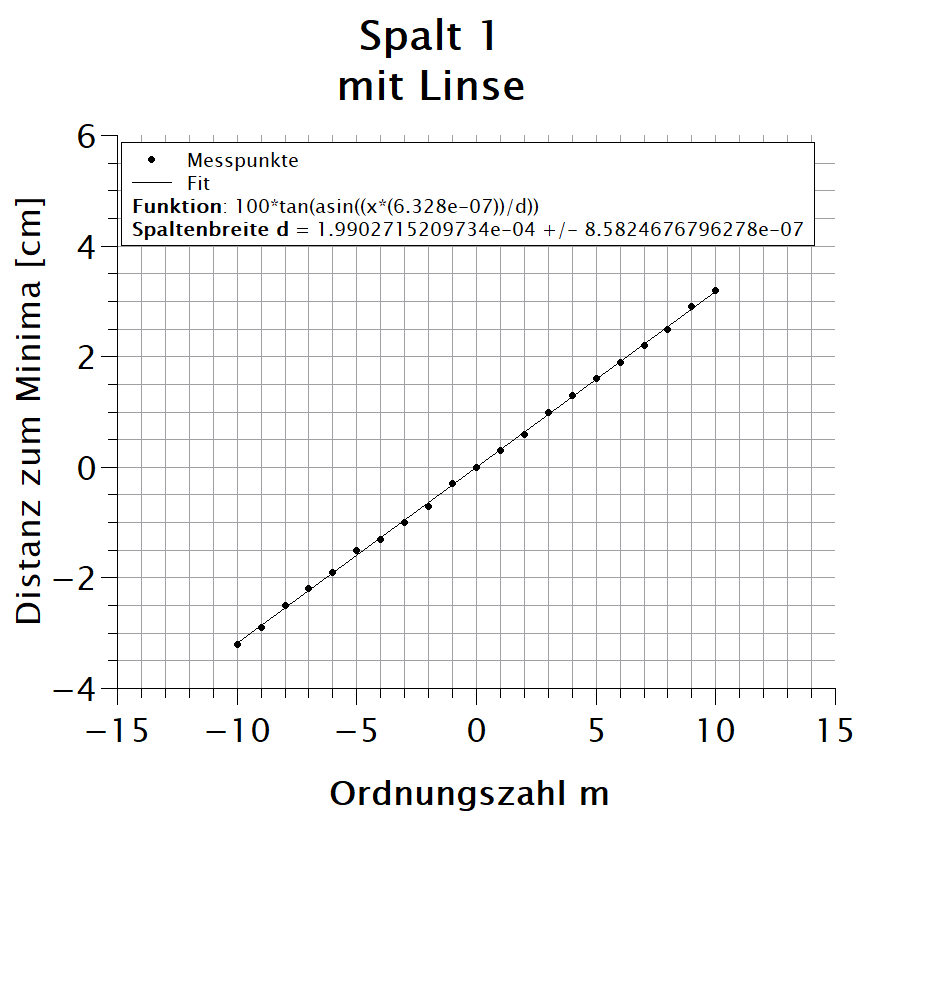
\includegraphics[width=\textwidth]{Bilder/spalt1_mitLinse.png} 
\vspace*{-3.5cm}
\caption[Spalt 1: mit Linse]{Hier wird der Abstand vom Mittelpunkt zum Minima des Interferenzmusters bei bestimmter Ordnungszahl, Frauenhofer'scher Beobachtungsart und mit Linse dargestellt. Dabei wird, wie in der Legende zu sehen ist, die Spaltenbreite gefittet. Es wurde zum Fit die Distanz von der Linse zum Schirm von 100cm verwendet.}
\label{fig:spalt1_mitLinse}
\end{figure}
\newpage

\begin{figure}[h]
\centering
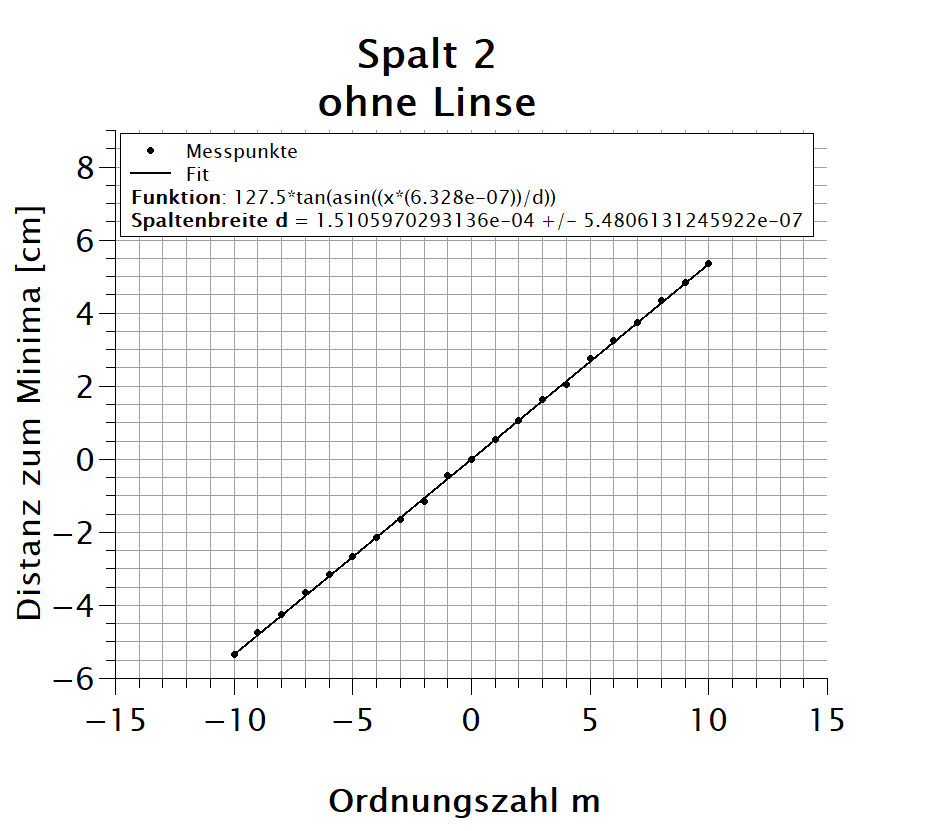
\includegraphics[width=\textwidth]{Bilder/spalt2_ohneLinse.png}
\vspace*{-1cm}
\caption[Spalt 2: ohne Linse]{Hier wird der Abstand vom Mittelpunkt zum Minima des Interferenzmusters bei bestimmter Ordnungszahl, direkter Beobachtung und ohne Linse dargestellt. Dabei wird, wie in der Legende zu sehen ist, die Spaltenbreite mit ihrem Fehler gefittet. Es wurde zum Fit die Distanz vom Objekt zum Schirm von 127.5cm verwendet.}
\label{fig:spalt2_ohneLinse}
\end{figure}
\newpage

\begin{figure}[h]
\centering
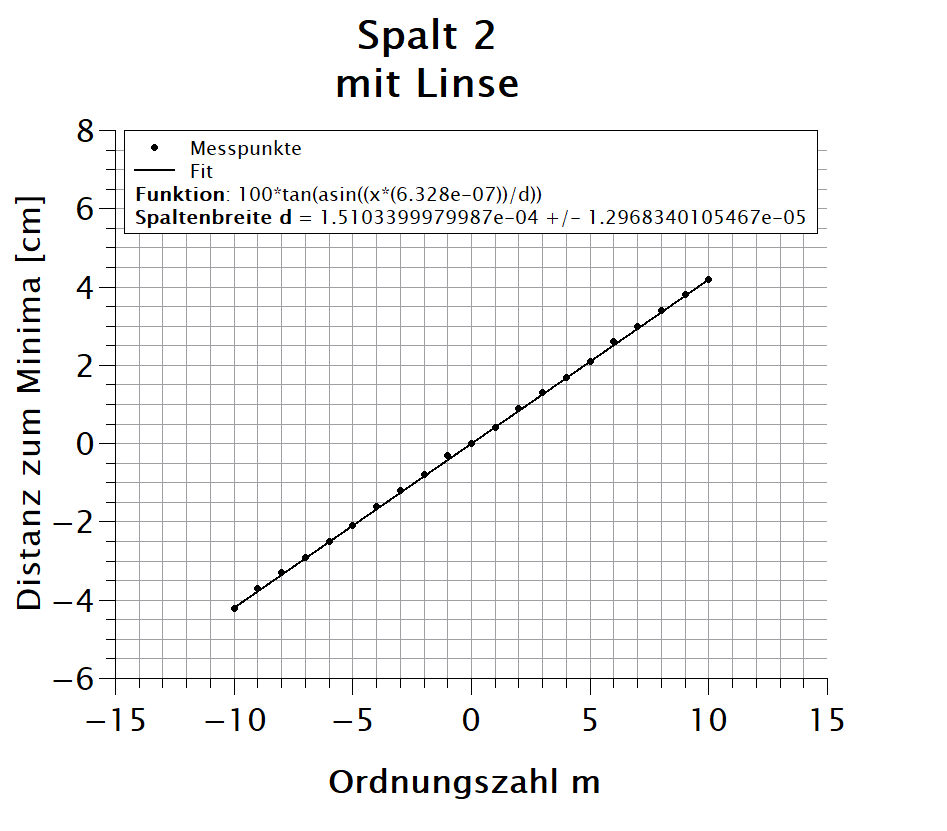
\includegraphics[width=\textwidth]{Bilder/spalt2_mitLinse.png} 
\vspace*{-1cm}
\caption[Spalt 2: mit Linse]{Hier wird der Abstand vom Mittelpunkt zum Minima des Interferenzmusters bei bestimmter Ordnungszahl, Frauenhofer'scher Beobachtungsart und mit Linse dargestellt. Dabei wird, wie in der Legende zu sehen ist, die Spaltenbreite gefittet. Es wurde zum Fit die Distanz von der Linse zum Schirm von 100cm verwendet.}
\label{fig:spalt2_mitLinse}
\end{figure}
\newpage

\begin{figure}[h]
\centering
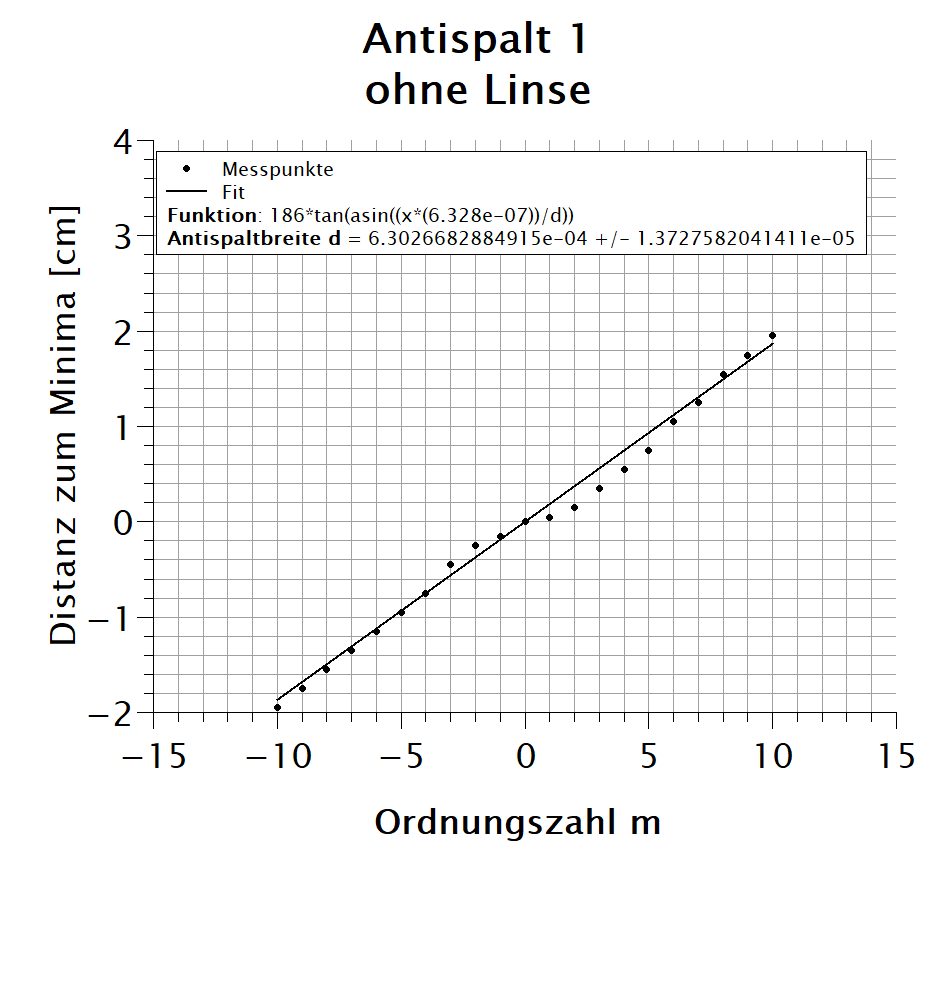
\includegraphics[width=\textwidth]{Bilder/antispalt1_ohneLinse.png}
\vspace*{-3.5cm}
\caption[Antispalt 1: ohne Linse]{Hier wird der Abstand vom Mittelpunkt zum Minima des Interferenzmusters bei bestimmter Ordnungszahl, direkter Beobachtung und ohne Linse dargestellt. Dabei wird, wie in der Legende zu sehen ist, die Spaltenbreite mit ihrem Fehler gefittet. Es wurde zum Fit die Distanz vom Objekt zum Schirm von 186cm verwendet.}
\label{fig:antispalt1_ohneLinse}
\end{figure}
\newpage

\begin{figure}[h]
\centering
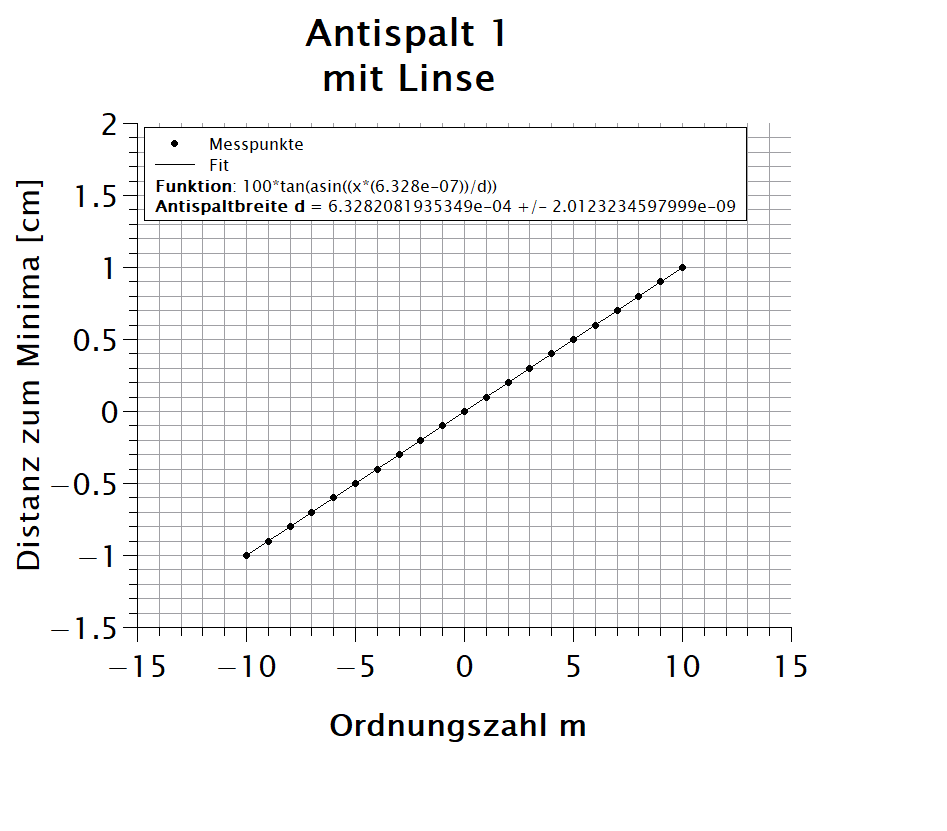
\includegraphics[width=\textwidth]{Bilder/antispalt1_mitLinse.png} 
\vspace*{-2cm}
\caption[Antispalt 1: mit Linse]{Hier wird der Abstand vom Mittelpunkt zum Minima des Interferenzmusters bei bestimmter Ordnungszahl, Frauenhofer'scher Beobachtungsart und mit Linse dargestellt. Dabei wird, wie in der Legende zu sehen ist, die Spaltenbreite gefittet. Es wurde zum Fit die Distanz von der Linse zum Schirm von 100cm verwendet.}
\label{fig:antispalt1_mitLinse}
\end{figure}
\newpage

\begin{figure}[h]
\centering
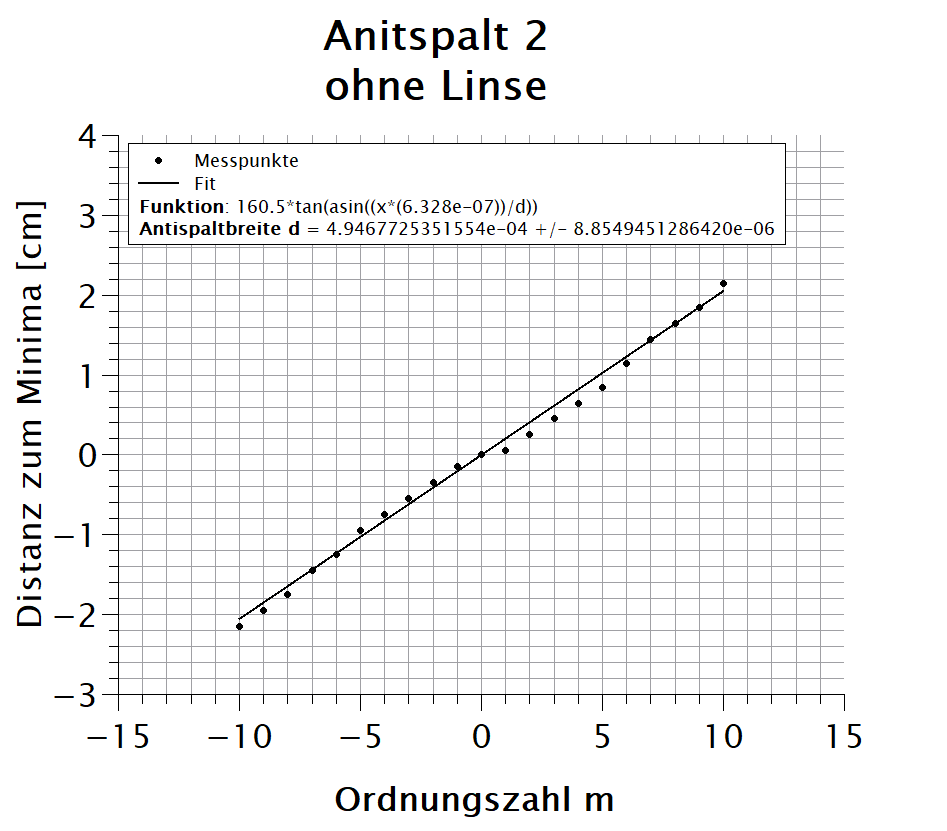
\includegraphics[width=\textwidth]{Bilder/antispalt2_ohneLinse.png}
\vspace*{-1cm}
\caption[Antispalt 2: ohne Linse]{Hier wird der Abstand vom Mittelpunkt zum Minima des Interferenzmusters bei bestimmter Ordnungszahl, direkter Beobachtung und ohne Linse dargestellt. Dabei wird, wie in der Legende zu sehen ist, die Spaltenbreite mit ihrem Fehler gefittet. Es wurde zum Fit die Distanz vom Objekt zum Schirm von 160.5cm verwendet.}
\label{fig:antispalt2_ohneLinse}
\end{figure}
\newpage

\begin{figure}[h]
\centering
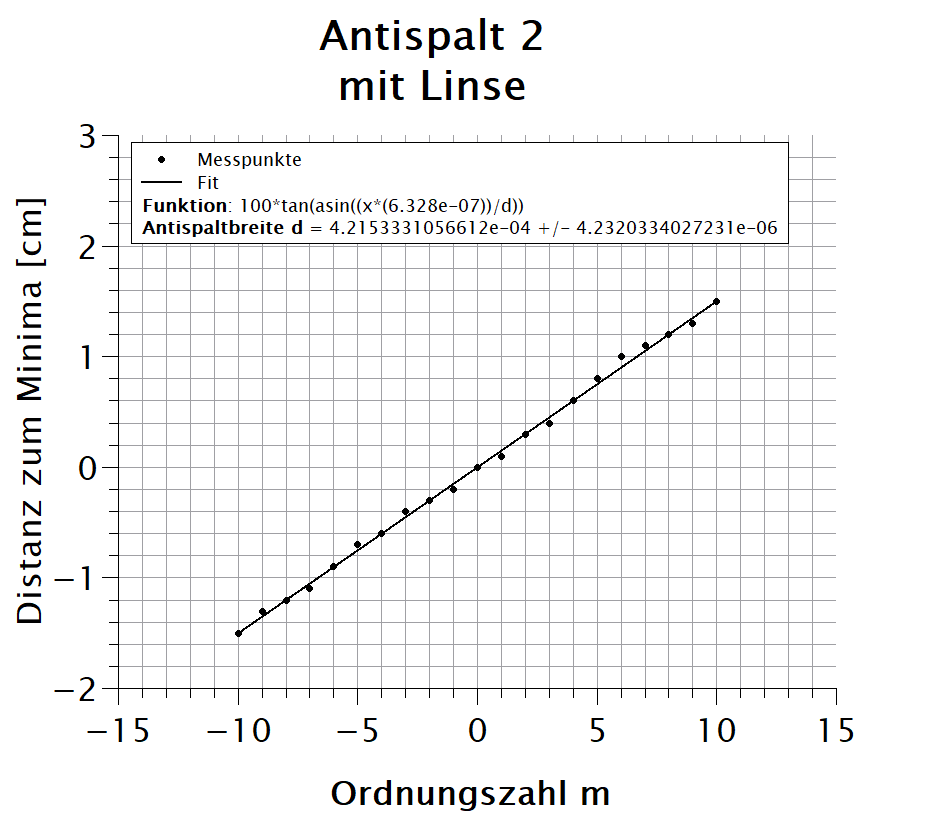
\includegraphics[width=\textwidth]{Bilder/antispalt2_mitLinse.png} 
\vspace*{-1cm}
\caption[Antispalt 2: mit Linse]{Hier wird der Abstand vom Mittelpunkt zum Minima des Interferenzmusters bei bestimmter Ordnungszahl, Frauenhofer'scher Beobachtungsart und mit Linse dargestellt. Dabei wird, wie in der Legende zu sehen ist, die Spaltenbreite gefittet. Es wurde zum Fit die Distanz von der Linse zum Schirm von 100cm verwendet.}
\label{fig:antispalt2_mitLinse}
\end{figure}
\newpage

\section{Beugung am Loch}
Hier werden die horizontal zum Mittelpunkt liegenden Minimas der Ringe des Interferenzmusters bestimmt. Nach der Gleichung \ref{eq:1} wird dann der Durchmesser des Loches gefittet. Nach Empfehlung des Dozenten wurde das Antiloch weggelassen.

\begin{figure}[h]
\centering
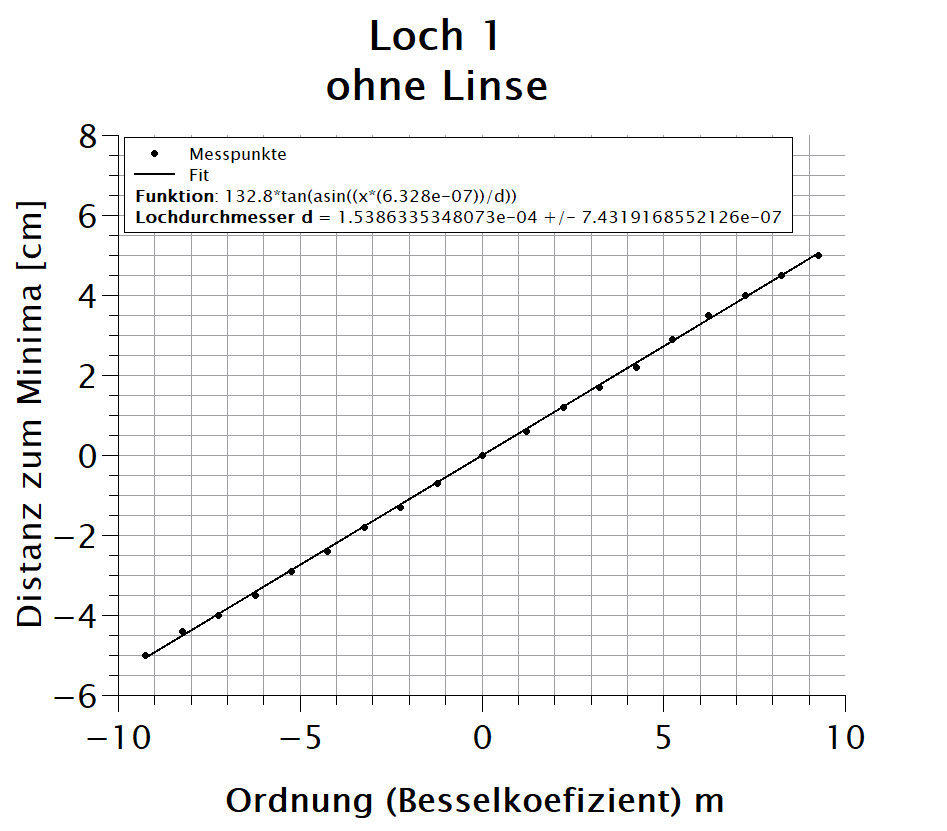
\includegraphics[width=\textwidth]{Bilder/loch1_ohneLinse.png} 
\caption[Loch 1: ohne Linse]{Hier repräsentiert jeder Messpunkt den Abstand vom Nullpunkt zum Minima der Ringe des Interferenzmusters nach dem Durchschreiten des He-Ne-Lasers durch das Loch mit direkter Beobachtungsart und ohne Linse. Dabei wurden für die Ordnung die bereits eruierten Koeffizienten verwendet. Als Abstand zum Schirm wurde die Distanz vom Objekt (Loch) zum Schirm direkt in die Gleichung \ref{eq:1} von 132.8cm eingefügt.}
\label{fig:loch1_ohneLinse}
\end{figure}
\newpage
\begin{figure}[h]
\centering
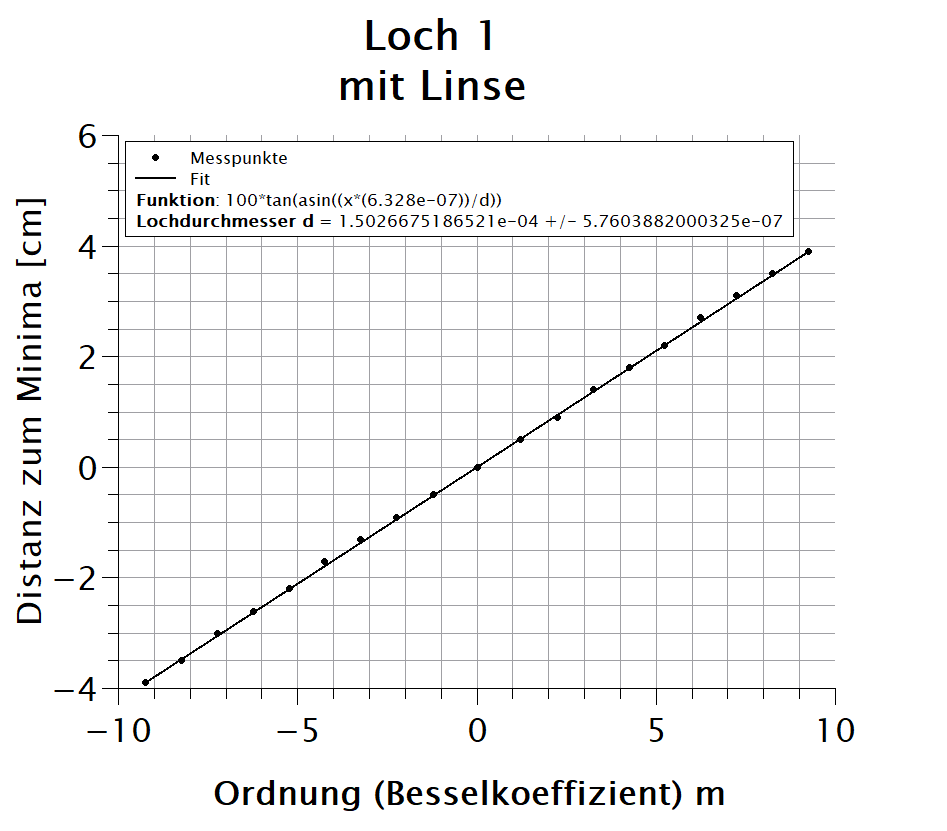
\includegraphics[width=\textwidth]{Bilder/loch1_mitLinse.png}  
\caption[Loch 1: mit Linse]{Hier repräsentiert jeder Messpunkt den Abstand vom Nullpunkt zum Minima der Ringe des Interferenzmusters nach dem Durchschreiten des He-Ne-Lasers durch das Loch mit Frauenhofer'scher Beobachtungsart und mit Linse. Dabei wurden für die Ordnung die bereits eruierten Koeffizienten verwendet. Als Abstand zum Schirm wurde die Distanz von der Linse zum Schirm direkt in die Gleichung \ref{eq:1} von 100cm eingefügt.}
\label{fig:loch1_mitLinse}
\end{figure}
\newpage

\begin{figure}[h]
\centering
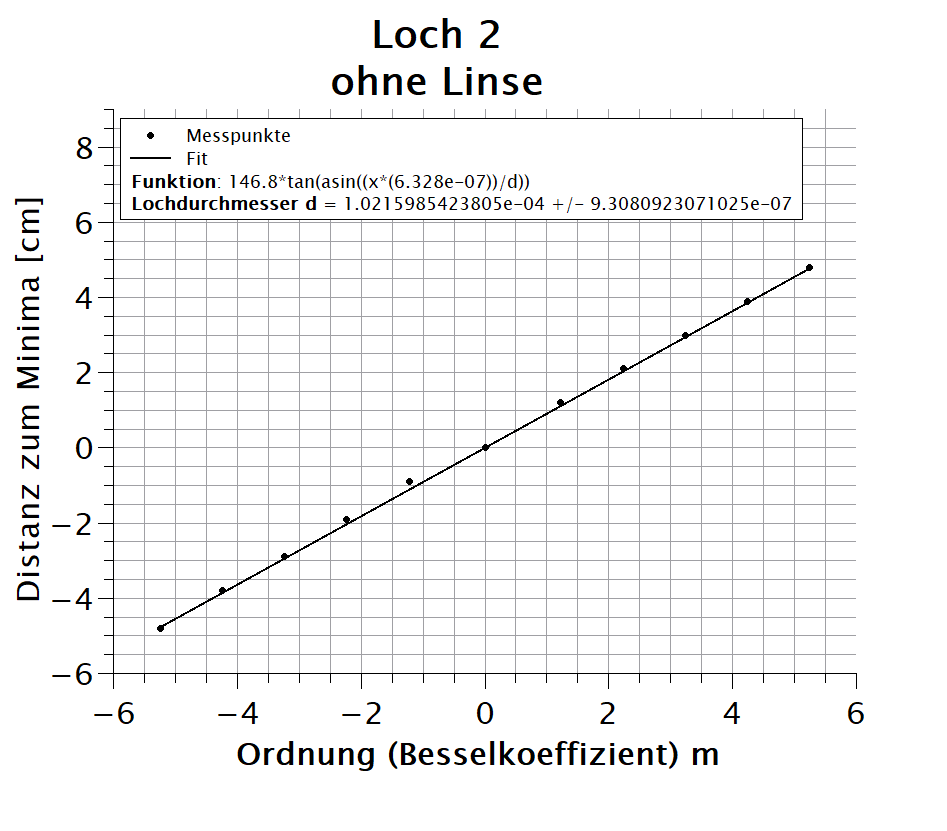
\includegraphics[width=\textwidth]{Bilder/loch2_ohneLinse.png} 
\caption[Loch 2: ohne Linse]{Hier repräsentiert jeder Messpunkt den Abstand vom Nullpunkt zum Minima der Ringe des Interferenzmusters nach dem Durchschreiten des He-Ne-Lasers durch das Loch mit direkter Beobachtungsart und ohne Linse. Dabei wurden für die Ordnung die bereits eruierten Koeffizienten verwendet. Als Abstand zum Schirm wurde die Distanz vom Objekt (Loch) zum Schirm direkt in die Gleichung \ref{eq:1} von 146.5cm eingefügt.}
\label{fig:loch2_ohneLinse}
\end{figure}
\newpage
\begin{figure}[h]
\centering
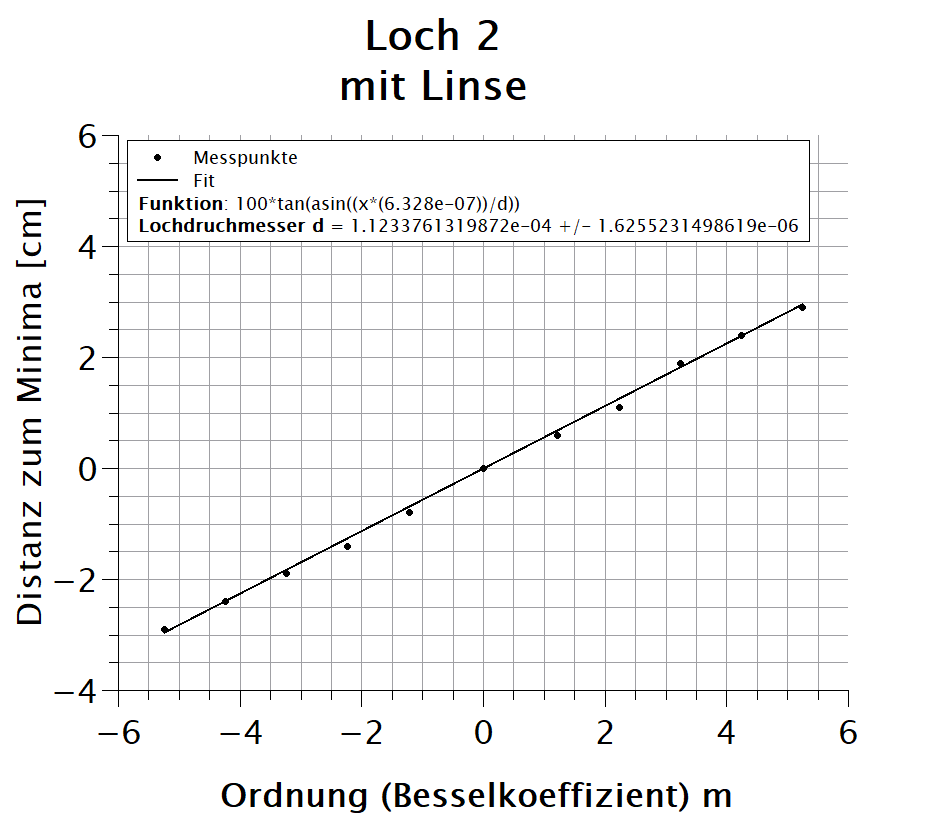
\includegraphics[width=\textwidth]{Bilder/loch2_mitLinse.png}  
\caption[Loch 2: mit Linse]{Hier repräsentiert jeder Messpunkt den Abstand vom Nullpunkt zum Minima der Ringe des Interferenzmusters nach dem Durchschreiten des He-Ne-Lasers durch das Loch mit Frauenhofer'scher Beobachtungsart und mit Linse. Dabei wurden für die Ordnung die bereits eruierten Koeffizienten verwendet. Als Abstand zum Schirm wurde die Distanz von der Linse zum Schirm direkt in die Gleichung \ref{eq:1} von 100cm eingefügt.}
\label{fig:loch2_mitLinse}
\end{figure}

\section{Beugung am Strichgitter}
Bei den Auswertungen/Messungen der Beugung des Lichts am Strichgitter traten Komplikationen auf, womit diese Ergebnisse zu keinem plausiblen Resultat führten. Die Plots sind im Anhang im im Kapitel \ref{sec:BeugungAmStrichgitter} \textit{\nameref{sec:BeugungAmStrichgitter}} zu finden
\newpage